%!TEX root = ./cikm2016.tex
\section{Experiments on \\ Knowledge Completion}
\label{sec:exp1}

\begin{table}[t]
\centering
\caption{\label{tbl:dataset}Description of datasets.
Sparsity denotes the ratio of valid triples to invalid triples.}
\vskip 0.15in
\begin{tabular}{l | r | r | r | r}
Dataset &  \# rel & \# entities & \# triples & sparsity \\ \hline
Kinship & 26 & 104  & 10,790 & 0.038 \\
UMLS & 49 &135  & 6,752 & 0.008 \\
Nation & 56 & 14  & 2,024 & 0.184 \\
%Wordnet & 11 & 38,696  &123,429 & 7.5e-06\\
%Wordnet(N) & 10 & 836 & 1,766 & 2.5e-04\\
\end{tabular}
\end{table}


\begin{figure}[t]
	\centering
	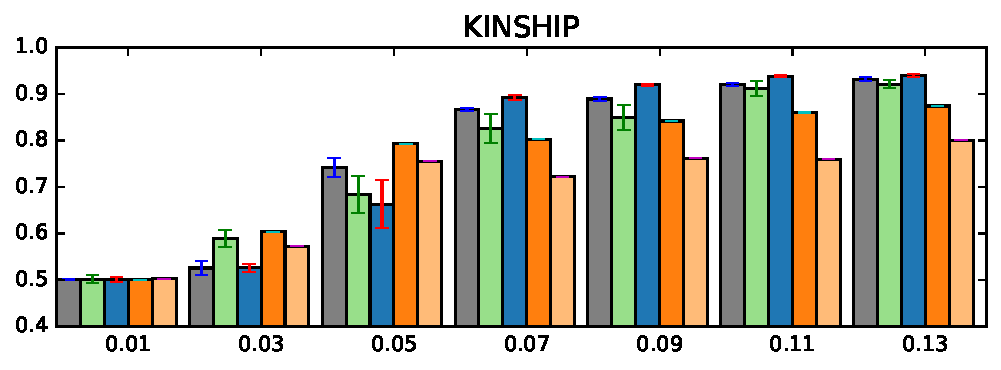
\includegraphics[width=\linewidth]{images/comp_training_error_kinship_small.pdf}
	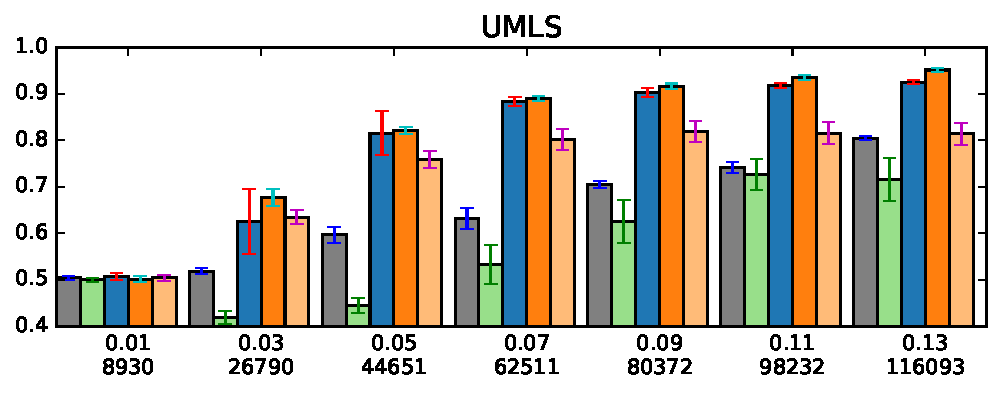
\includegraphics[width=\linewidth]{images/comp_training_error_umls_small.pdf}
	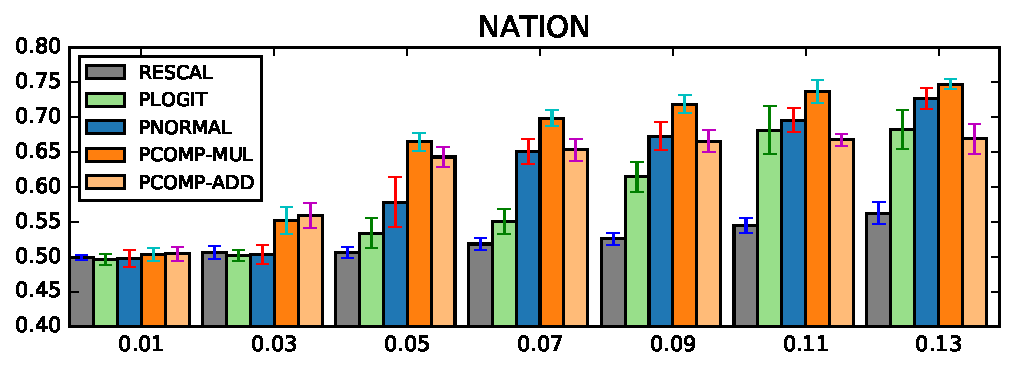
\includegraphics[width=\linewidth]{images/comp_training_error_nation_small.pdf}
	\caption{\label{fig:r_vs_br} ROC-AUC scores of compositional models.
	The x-axis denotes the proportion and total number of triples used for training. %We use other 20\% of triples as a validation set and another 30\% of triples as a test set.
}
\end{figure}

\begin{figure}[t]
	\centering
	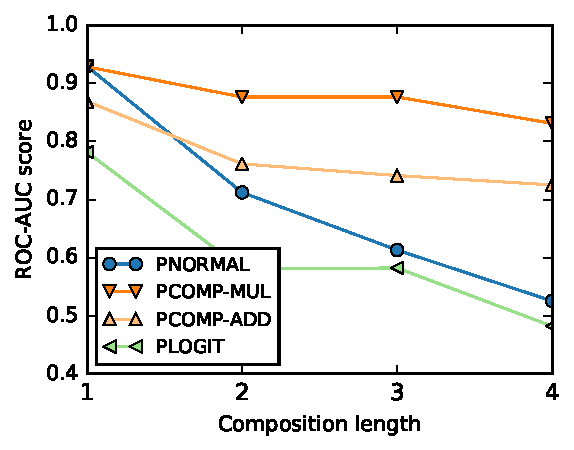
\includegraphics[width=0.9\linewidth]{images/path_prediction2.pdf}
	\caption{\label{fig:path_pred} Path prediction result with UMLS.
	The performances of both compositional models remain consistent
	whereas those of the non-compositional models drop sharply as the length increases.}
\end{figure}


\begin{table*}[t]
\small
\center
\caption{\label{tbl:path_example} Example of path prediction from UMLS data. We predict top 5 entities in compositional triples starting from entity \texttt{Mental-or-Behavioral (MB) Dysfunction} followed by two relations \texttt{Affects} and \texttt{Produces}. Correct entities are bolded.}

\subfigure[Triple prediction: \texttt{(MB Dysfunction, Affects, -)}]{
\begin{tabular}{l | p{2.7cm}p{2.7cm}p{2.7cm}p{2.7cm}p{2.7cm}}
Model & Top 1 & Top 2 & Top 3 & Top 4 & Top 5 \\ \hline \hline
\textsc{Pnormal} & \textbf{Invertebrate}&\textbf{Reptile}&\textbf{Archaeon}&\textbf{Bird}&\textbf{Phy.-Function} \\ \hline
\textsc{Plogit} & \textbf{Cell-Function}&\textbf{Disease-or-Syndrome}&\textbf{Cell-or-Molecular-Dysf.}&\textbf{Exp.-Model-of-Disease}&\textbf{Mental-Process} \\ \hline
\textsc{Pcomp-mul} & \textbf{Archaeon}&\textbf{Fish}&\textbf{Fungus}&\textbf{Invertebrate}&\textbf{Human} \\ \hline
\textsc{Pcomp-add} & \textbf{Path.-Function}&\textbf{Bird}&\textbf{Cell-or-Molecular-Dysf.}&Drug-Delivery-Device&Congenital-Abnormality

\end{tabular}
}
\subfigure[Length-2 path prediction: \texttt{(MB Dysfunction, Affects, Produces, -)}]{
\begin{tabular}{l | p{2.7cm}p{2.7cm}p{2.7cm}p{2.7cm}p{2.7cm}}
Model & Top 1 & Top 2 & Top 3 & Top 4 & Top 5 \\ \hline \hline
\textsc{Pnormal} & Clinical-Drug&Sign-or-Symptom&Org.-Attribute&Drug-Delivery-Device&Clinical-Attr. \\ \hline
\textsc{Plogit} & Amphibian&Gov.-or-Reg.-Activity&Food&Biologic-Func.&Classification\\ \hline
\textsc{Pcomp-mul} & \textbf{Enzyme}&\textbf{Body-Substance}&\textbf{Biogenic-Amine}&Carbohydrate&\textbf{Immunologic-Factor} \\ \hline
\textsc{Pcomp-add} & \textbf{Immunologic-Factor}&\textbf{Body-Substance}&Molecular-Biology-Research-Technique&Clinical-Drug&Chemical-Viewed-Structurally

\end{tabular}
}
\end{table*}


%\begin{figure}[t]
%	\centering
%	\includegraphics[width=\linewidth]{images/path_reconstruction.pdf}
%	\caption{\label{fig:path_pred_example} Example of path-prediction from UMLS. From entity \texttt{Mental-or-Behavioral Dysfunction}, we predict entities after two relations \texttt{Affects}/\texttt{Produces} with different models. Y-axis indicates an ROC-AUC score after each prediction. Labels of x-axis show reachable entities after each relation.}
%\end{figure}

%Applying Thompson sampling to the compositional models is not straight forward.
%Because, in the compositional model, adding one valid triple in a knowledge base will
%change the accompanying compositional paths over the extended tensor $\mathcal{X}^L$.
%Therefore, the system requires to compute potential changes in the
%compositional structure for every candidate query triple. This computational complexity
%will increase exponentially as we increase the length of the composition.

%In this experiment, instead running the Thompson sampling for the compositional models,
We first evaluate our model for the knowledge completion task
%we follow the standard train/validation/test approach
to measure the predictive performance of \textsc{Prescal} with all non compositional and compositional variants.
%The results between active acquisition and training and testing are not always coincident, but if the Thompson sampling samples latent features from true posterior of the compositional model, the samples corresponds to the true posterior samples from the training set.
We evaluate the models on three benchmark datasets\footnote{https://alchemy.cs.washington.edu/papers/kok07/}: KINSHIP, UMLS, and NATION, and compare  performances with the original \textsc{RESCAL}. 
Detailed description of each
dataset is shown in Table \ref{tbl:dataset}.

\begin{figure*}[t]
	\centering

%	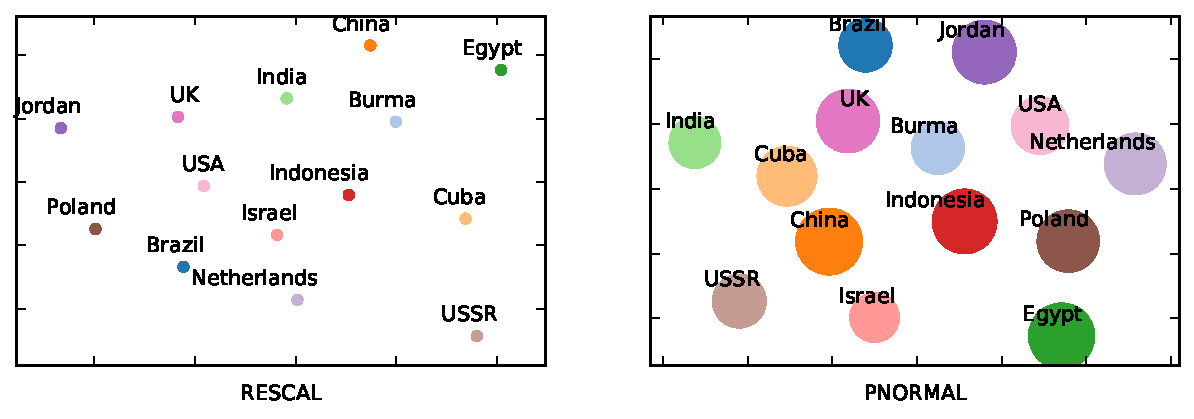
\includegraphics[width=0.7\linewidth]{images/embedding_nation.pdf}
	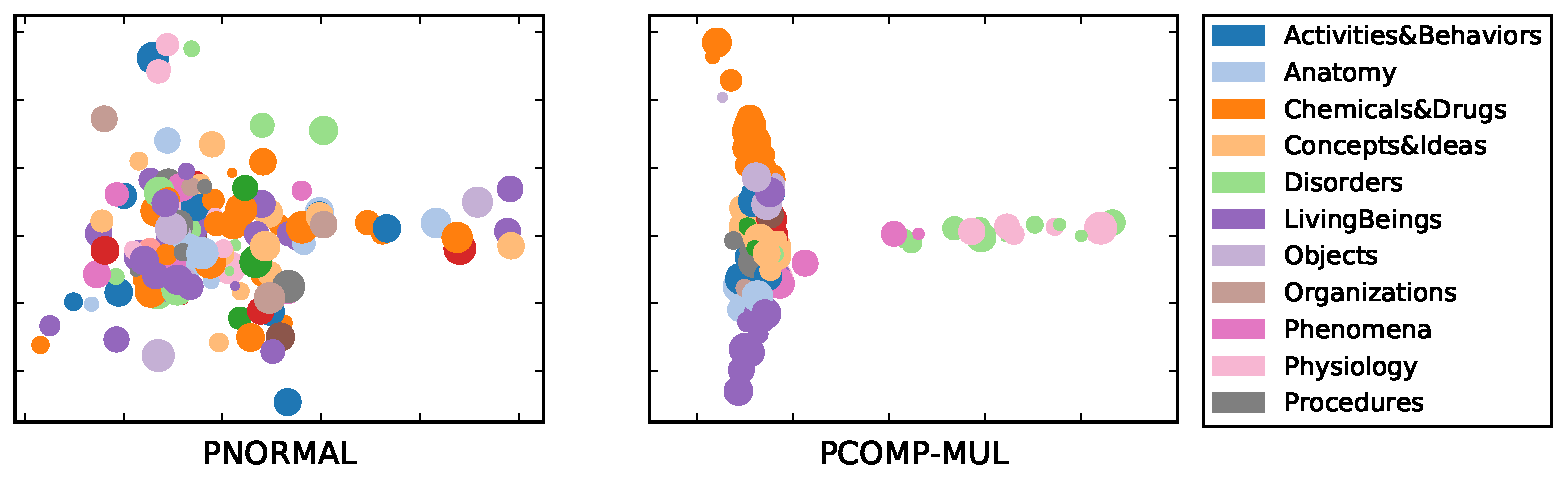
\includegraphics[width=0.7\linewidth]{images/embedding_umls.pdf}

	\caption{\label{fig:tsne} Embedding learned entities of the UMLS dataset into a two-dimensional space through the spectral clustering. Entities with the same type are represented by the same color.}
\end{figure*}

For all experiments, we set the compositional length $L$ to 2, split the dataset into 20\% for validation and 30\% for testing. We vary the proportion of training triples
from 1\% to 13\% of datasets. For \textsc{Rescal}, we use the authors' implementation\footnote{https://github.com/mnick/rescal.py}, and measure performance over 10 runs with random initialisations. For \textsc{Prescal} and all the variants, we sample triples $x_{ikj}$ from its posterior, and measure performance over 10 different samples.
%Based on the trained model, measure the ROC-AUC scores on the test set.
The performances of models are measured by ROC-AUC score on the test set:
\begin{align}
\frac{1}{|\mathcal{X}_p|  |\mathcal{X}_n|} \sum_{\{i,k,j\} \in \mathcal{X}_p, \{i',k',j'\} \in \mathcal{X}_n} \mathbb{I}[\bar{x}_{ikj} > \bar{x}_{ikj}],
\end{align}
where $\mathcal{X}_p$ and $\mathcal{X}_n$ are the set of positive and negative triples in the test set, respectively, and $\bar{x}$ is a reconstructed triple.

Figure \ref{fig:r_vs_br} shows the ROC-AUC scores of the compositional models
with the various baseline models. We can see that the \textsc{Prescal} with
the normal output (\textsc{Pnormal}) or logistic output (\textsc{Plogit}) generally outperform \textsc{Rescal}.
We compare the compositional model with original \textsc{Rescal}, \textsc{Pnormal}, and \textsc{Plogit}.
In general, the multiplicative compositional model (\textsc{Pcomp-mul}) outperforms
the additive compositional model (\textsc{Pcomp-add}), and performs better than the other baseline models
when the proportion of training set is small. For UMLS and NATION, \textsc{Pcomp-mul} outperforms
across the all training proportions.
For KINSHIP, however, the model performs better when the training proportion is less than 7\%.

The goal of the compositional models is to factorise triples along with the graph structure as a whole.
The triple prediction task tells us the trained model is capable of triple prediction,
but does not tell whether the features can recover the graph structure.
%Both models perform well in triple prediction, but this does not tell
If the model factorises the graph structure properly,
then the trained model can predict not only triples but the graph structure as well.
To validate the model assumption, we evaluate a path prediction task.
For this task, we use 10\% of UMLS dataset for training.
We compute the expected value of unobserved path given a trained model.
The non-compositional models are not capable to compute the expected value.
In such a case, we approximate paths with multiplicative model assumption in Equation \ref{eqn:multi}.
We vary the path length from 1 (triple) to 4, and measure ROC-AUC scores on the reconstructed compositional triples.
Figure \ref{fig:path_pred} shows the result.
Both compositional models show consistent performance regardless of the path length.
However, the performance of the non-compositional models drops sharply as the length increases.
The results show the compositional models preserve a graph structure in the embedded space.
It is worth emphasising that although the compositional length for training is 2,
the compositional models show consistent results on predicting path of length 3 and 4.

Table \ref{tbl:path_example} shows an example of the path prediction result
starting from entity \texttt{Mental-or-Behavioral (MB) Dysfunction} followed by two relations \texttt{Affects} and \texttt{Produces}.
Both compositional and non-compositional models predict triples well.
For length-2 path prediction, only the compositional models can capture correct entities on top 5.
We also visualise the multi-dimensional entities inferred by \textsc{Pnormal} and \textsc{Pcomp-mul}
into a two-dimensional space through the spectral clustering \cite{von2007tutorial}
in Figure \ref{fig:tsne}.
A circle represents an entity,
and the size of the circle is proportional to the uncertainty of the entity in the latent space.
In the UMLS dataset, the entities are categorised into 15 types,
e.g. \texttt{Disorders}, \texttt{Living-Beings}, \texttt{Phenomena}, etc.
We use the same color to represent the entities with the same type.
The entities with the same type are located closer to each other with \textsc{Pcomp-mul} than \textsc{Pnormal}.
